%
% ---------------------------------------------------------------
% Copyright (C) 2012-2018 Gang Li
% ---------------------------------------------------------------
%
% This work is the default powerdot-tuliplab style test file and may be
% distributed and/or modified under the conditions of the LaTeX Project Public
% License, either version 1.3 of this license or (at your option) any later
% version. The latest version of this license is in
% http://www.latex-project.org/lppl.txt and version 1.3 or later is part of all
% distributions of LaTeX version 2003/12/01 or later.
%
% This work has the LPPL maintenance status "maintained".
%
% This Current Maintainer of this work is Gang Li.
%
%

\documentclass[
size=14pt,
paper=smartboard,  %a4paper, smartboard, screen
mode=present, 		%present, handout, print
display=slides, 	% slidesnotes, notes, slides
style=tuliplab,  	% TULIP Lab style
pauseslide,
fleqn,leqno]{powerdot}


\usepackage{cancel}
\usepackage{caption}
\usepackage{stackengine}
\usepackage{smartdiagram}
\usepackage{attrib}
\usepackage{amssymb}
\usepackage{amsmath} 
\usepackage{amsthm} 
\usepackage{mathtools}
\usepackage{rotating}
\usepackage{graphicx}
\usepackage{boxedminipage}
\usepackage{rotate}
\usepackage{calc}
\usepackage[absolute]{textpos}
\usepackage{psfrag,overpic}
\usepackage{fouriernc}
\usepackage{pstricks,pst-3d,pst-grad,pstricks-add,pst-text,pst-node,pst-tree}
\usepackage{moreverb,epsfig,subfigure}
\usepackage{color}
\usepackage{booktabs}
\usepackage{etex}
\usepackage{breqn}
\usepackage{multirow}
\usepackage{natbib}
\usepackage{bibentry}
\usepackage{gitinfo2}
\usepackage{siunitx}
\usepackage{nicefrac}
%\usepackage{geometry}
%\geometry{verbose,letterpaper}
\usepackage{media9}
\usepackage{animate}
%\usepackage{movie15}
\usepackage{auto-pst-pdf}

\usepackage{breakurl}
\usepackage{fontawesome}
\usepackage{xcolor}
\usepackage{multicol}



\usepackage{verbatim}
\usepackage[utf8]{inputenc}
\usepackage{D:/texlive/2022/dtk-logos}
\usepackage{tikz}
\usepackage{adigraph}
%\usepackage{tkz-graph}
\usepackage{hyperref}
%\usepackage{ulem}
\usepackage{pgfplots}
\usepackage{verbatim}
\usepackage{fontawesome}


\usepackage{todonotes}
% \usepackage{pst-rel-points}
\usepackage{animate}
\usepackage{fontawesome}

\usepackage{listings}
\lstset{frameround=fttt,
	frame=trBL,
	stringstyle=\ttfamily,
	backgroundcolor=\color{yellow!20},
	basicstyle=\footnotesize\ttfamily}
\lstnewenvironment{code}{
	\lstset{frame=single,escapeinside=`',
		backgroundcolor=\color{yellow!20},
		basicstyle=\footnotesize\ttfamily}
}{}


\usepackage{hyperref}
\hypersetup{ % TODO: PDF meta Data
	pdftitle={Presentation Title},
	pdfauthor={Gang Li},
	pdfpagemode={FullScreen},
	pdfborder={0 0 0}
}


% \usepackage{auto-pst-pdf}
% package to show source code

\definecolor{LightGray}{rgb}{0.9,0.9,0.9}
\newlength{\pixel}\setlength\pixel{0.000714285714\slidewidth}
\setlength{\TPHorizModule}{\slidewidth}
\setlength{\TPVertModule}{\slideheight}
\newcommand\highlight[1]{\fbox{#1}}
\newcommand\icite[1]{{\footnotesize [#1]}}

\newcommand\twotonebox[2]{\fcolorbox{pdcolor2}{pdcolor2}
	{#1\vphantom{#2}}\fcolorbox{pdcolor2}{white}{#2\vphantom{#1}}}
\newcommand\twotoneboxo[2]{\fcolorbox{pdcolor2}{pdcolor2}
	{#1}\fcolorbox{pdcolor2}{white}{#2}}
\newcommand\vpspace[1]{\vphantom{\vspace{#1}}}
\newcommand\hpspace[1]{\hphantom{\hspace{#1}}}
\newcommand\COMMENT[1]{}

\newcommand\placepos[3]{\hbox to\z@{\kern#1
		\raisebox{-#2}[\z@][\z@]{#3}\hss}\ignorespaces}

\renewcommand{\baselinestretch}{1.2}


\newcommand{\draftnote}[3]{
	\todo[author=#2,color=#1!30,size=\footnotesize]{\textsf{#3}}	}
% TODO: add yourself here:
%
\newcommand{\gangli}[1]{\draftnote{blue}{GLi:}{#1}}
\newcommand{\shaoni}[1]{\draftnote{green}{sn:}{#1}}
\newcommand{\gliMarker}
{\todo[author=GLi,size=\tiny,inline,color=blue!40]
	{Gang Li has worked up to here.}}
\newcommand{\snMarker}
{\todo[author=Sn,size=\tiny,inline,color=green!40]
	{Shaoni has worked up to here.}}

%%%%%%%%%%%%%%%%%%%%%%%%%%%%%%%%%%%%%%%%%%%%%%%%%%%%%%%%%%%%%%%%%%%%%%%%
% title
% TODO: Customize to your Own Title, Name, Address
%
\title{April Tabular Playground Series - Your Baseline Model}
\author{
	Jinzhu Liu
	\\
	\\Nanjing University of Science and Technology
	\\Deakin University, Australia
}
\date{\gitCommitterDate}


% Customize the setting of slides
\pdsetup{
	% TODO: Customize the left footer, and right footer
	rf=\href{http://www.tulip.org.au}{
		Last Changed by: \textsc{\gitCommitterName}\ \gitVtagn-\gitAbbrevHash\ (\gitAuthorDate)
	},
	cf={April Tabular Playground Series - Your Baseline Model},
}


\begin{document}
	
	\maketitle
	
	%\begin{slide}{Overview}
	%\tableofcontents[content=sections]
	%\end{slide}
	
	
	%%==========================================================================================
	%%
	\begin{slide}[toc=,bm=]{Overview}
		\tableofcontents[content=currentsection,type=1]
	\end{slide}
	%%
	%%==========================================================================================
	
	
	\section{Problem Definition}
	
	
	%%==========================================================================================
	%%
	\begin{slide}{Predict Whether or not A Passenger Survived the Inking of the Synthanic}
		\begin{center}
			\twotonebox{\rotatebox{90}{Introduce}}{\parbox{1\textwidth}
				{it is extremely important to start somewhere and identify it as your first standard of comparision against the progress you have.This helps you make a baseline model, get a baseline score.
					\begin{itemize}
						\item We task is to predict whether or not a passenger survived the sinking of the Synthanic.
					\end{itemize}
			}}
		\end{center}
		\begin{center}
			\twotonebox{\rotatebox{90}{Interpretation}}{\parbox{1\textwidth}
				{Variable Notes
					\begin{itemize}
						\item pclass: A proxy for socio-economic status (SES) 1st = Upper 2nd = Middle 3rd = Lower \\
						age: Age is fractional if less than 1. If the age is estimated, is it in the form of xx.5 \\
						sibsp: TDescribes the number of Siblings and spouses accompanying passengers on the Titanic \\
						parch: Describes the number of parents and children travelling with passengers on the Titanic
					\end{itemize}
			}}
			
		\end{center}
		\bigskip
		
		
	\end{slide}
	%%
	%%==========================================================================================
	
	
	%%==========================================================================================
	%%
	\begin{slide}[toc=,bm=]{Predict Whether or not A Passenger Survived the Inking of the Synthanic}
		\begin{center}
			\begin{tabular}{c| c c c c c c c}
				\toprule
				%\centering
				{} & \texttt{Passengerid}  & \texttt{Survived} & \texttt{Pclass} & \texttt{Name}  & \texttt{Sex} & \texttt{Age}  & \texttt{SibSp} \\
				\midrule
				$0$
				&  {$0$} &  {$1$} &  {$1$} &  {Oconnor, Frankie} &  {male} &  {NaN} &  {$2$} \\
				$1$
				&  {$1$} &  {$0$}&  {$3$}&  {Bryan, Drew} &  {male} &  {NaN} &  {$0$} \\
				$2$
				&  {$2$} &  {$0$} &  {$3$} &  {Owens, Kenneth} &  {male} &  {$0.33$} &  {$1$} \\
				$3$
				&  {$3$} &  {$0$}&  {$3$}&  {Kramer, James} &  {male} &  {$19.00$} &  {$0$} \\
				$4$
				&  {$4$} &  {$1$} &  {$3$} &  {Bond, Michael} &  {male} &  {$25.00$} &  {$0$} \\
				\bottomrule
			\end{tabular}
		\end{center}
		\begin{center}
			\begin{tabular}{c| c c c c c}
				\toprule
				%\centering
				{} & \texttt{Parch} & \texttt{Ticket}  & \texttt{Fare} & \texttt{Cabin}  & \texttt{Embarked}\\
				\midrule
				$0$
				&  {$0$} &  {$209245$} &  {$27.14$} &  {C$12239$} &  {S} \\
				$1$
				&  {$0$} &  {$27323$} &  {$13.35$} &  {NaN} &  {S} \\
				$2$
				&  {$2$} &  {CA$457703$} &  {$71.29$} &  {NaN} &  {S} \\
				$3$
				&  {$0$} &  {A$.10866$} &  {$13.04$} &  {NaN} &  {S} \\
				$4$
				&  {$0$} &  {$427635$} &  {$7.76$} &  {NaN} &  {S} \\
				\bottomrule
			\end{tabular}
		\end{center}
	\end{slide}
	%%
	%%==========================================================================================
	
	
	%%==========================================================================================
	%%
	
	
	\section{Data analysis and processing}
	
	
	%%==========================================================================================
	%%
	\begin{slide}{Inquire NaN Values}
		\begin{center}	\begin{tabular}{c|c}
				\toprule
				%\centering
				\midrule
				{PassengerId}
				&  {$0$} \\
				{Survived}
				&  {$0$} \\
				{Pclass}
				&  {$0$} \\
				{Name}
				&  {$0$} \\
				{Sex}
				&  {$3292$} \\
				{Age}
				&  {$0$} \\
				{SibSp}
				&  {$0$} \\
				{Parch}
				&  {$0$} \\
				{Ticket}
				&  {$4623$} \\
				{Fare}
				&  {$134$} \\
				{Cabin}
				&  {$67866$} \\
				{Embarked}
				&  {$250$} \\
				\bottomrule
			\end{tabular}
		\end{center}
		\vspace{-0.6cm}
		\begin{itemize}
			\item
			list out the columns holding Numerical Values - \textcolor{orange}{1.Age  2.Fare}
			\item
			The remaining columns do not hold numerical values. Let's explore the distribution of the numerical values a bit before we replace their NaN values
		\end{itemize}
	\end{slide}
	%%
	%%==========================================================================================
	
	
	%%==========================================================================================
	%%
	\begin{slide}{Studying Distribution of Age and Fare}
		\vspace{-0.8cm}
		Fare
		\vspace{-0.8cm}
		\begin{figure}
			\centering
			\selectcolormodel{rgb}
			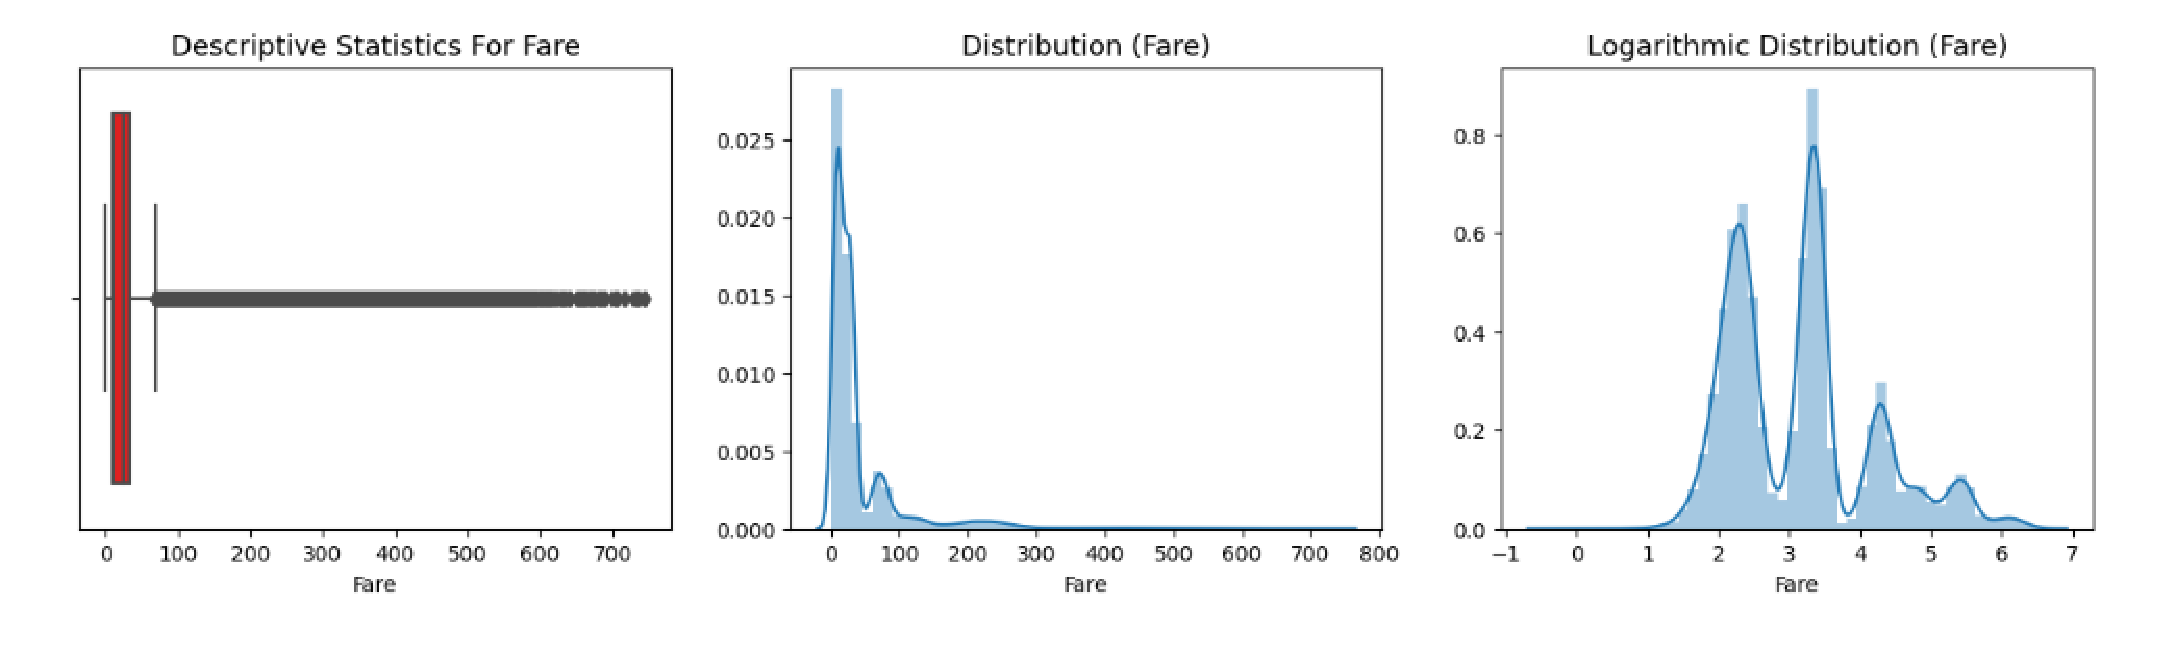
\includegraphics[width=1\textwidth]{figures//fig1.eps}\\
			\caption{Descriptive Statistics For Fare}
		\end{figure}
		\vspace{-0.8cm}
		\begin{itemize}
			\item
			From the boxplot , we can see that anything above 100 looks like an outlier and that there are a lot of outliers. The suggested median seems to be somewhere between 0-100.
			\item
			The Distribution Plot suggests that the data is left skewed.
			\item 
			From the Logarithmic Distribution,we can assume that these three peaks are a result of price distribution on those three classes.
		\end{itemize}
	\end{slide}
	%%
	%%==========================================================================================
	
	
	%%==========================================================================================
	%%
	\begin{slide}[toc=,bm=]{Fare distribution for each class}
		\vspace{-1cm}
		\begin{figure}
			\centering
			\selectcolormodel{rgb}
			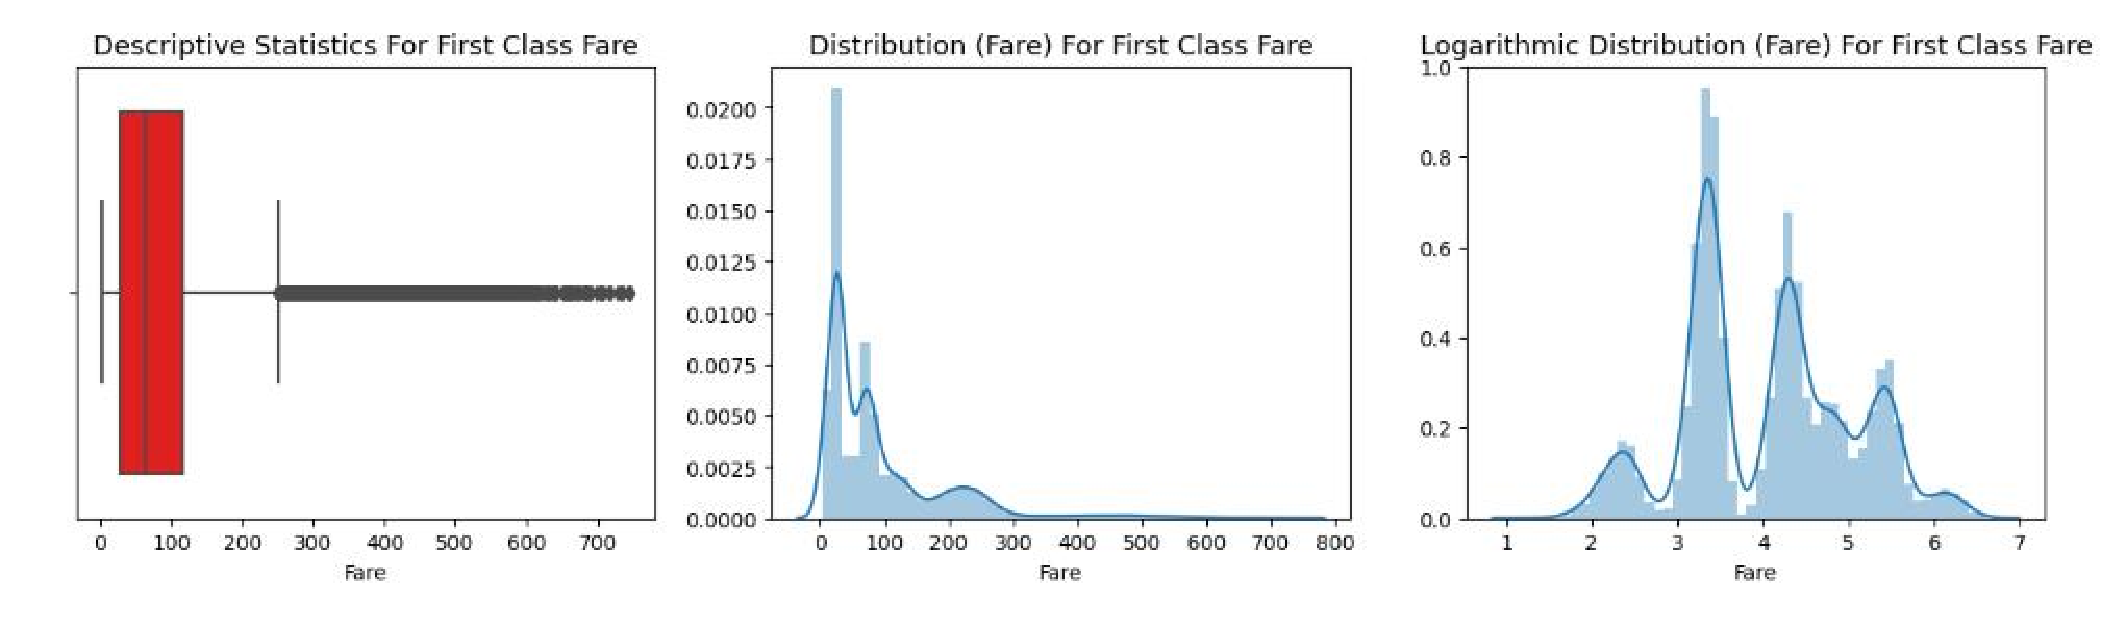
\includegraphics[width=1\textwidth]{figures//fig2.eps}\\
			\vspace{-0.4cm}
			\caption{First Class Fare}
		\end{figure}
		\vspace{-1.2cm}
		\begin{figure}
			\centering
			\selectcolormodel{rgb}
			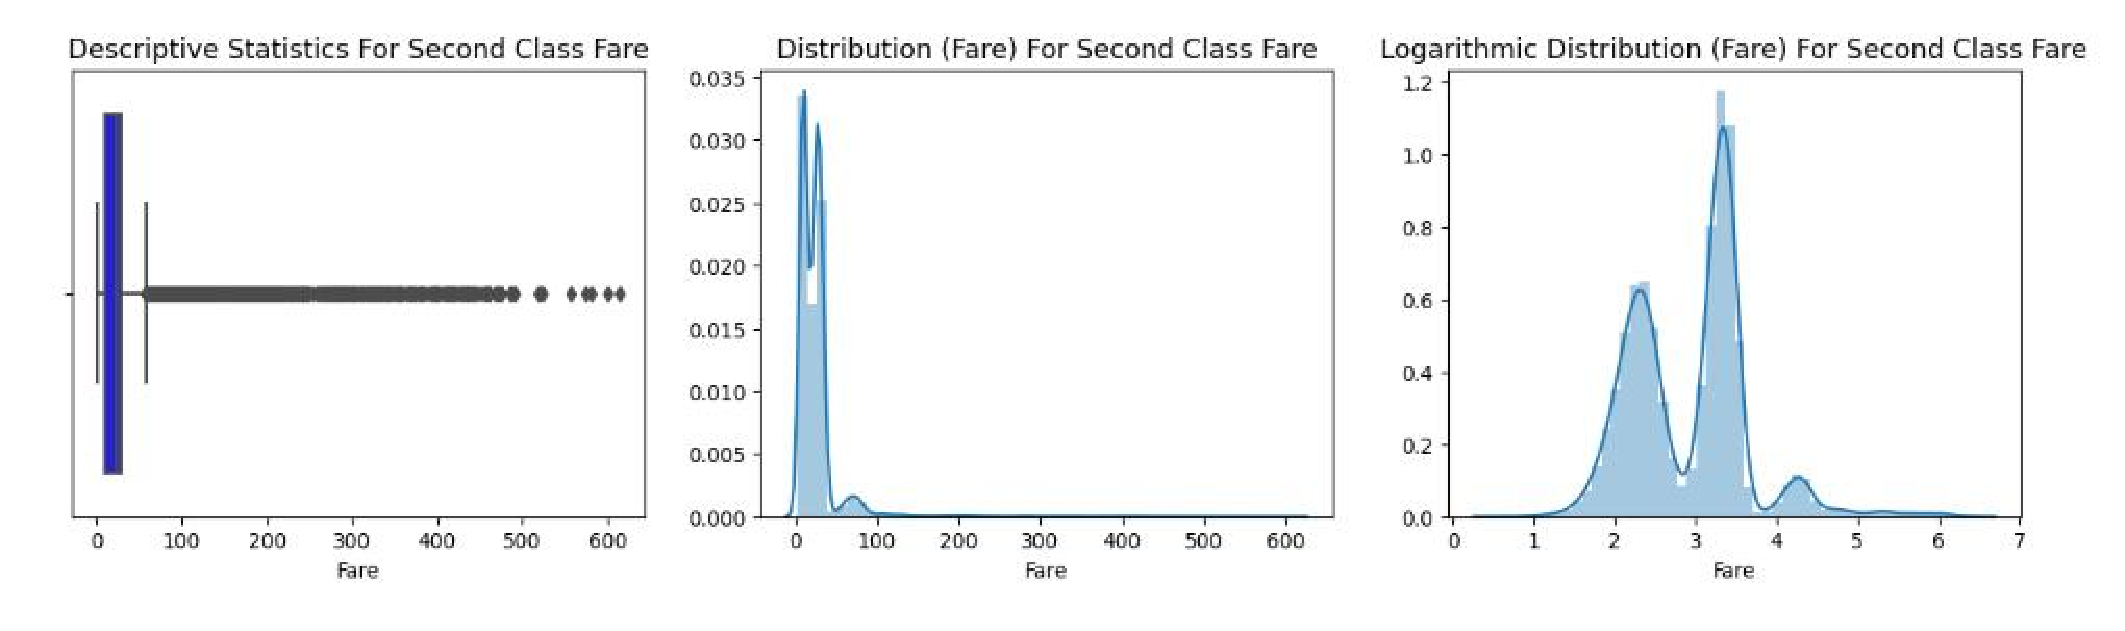
\includegraphics[width=1\textwidth]{figures//fig3.eps}\\
			\vspace{-0.4cm}
			\caption{Second Class Fare}
		\end{figure}
	\end{slide}
	%%
	%%==========================================================================================
	
	
	%%==========================================================================================
	%%
	\begin{slide}[toc=,bm=]{}
		\vspace{-0.8cm}
		\begin{figure}
			\centering
			\selectcolormodel{rgb}
			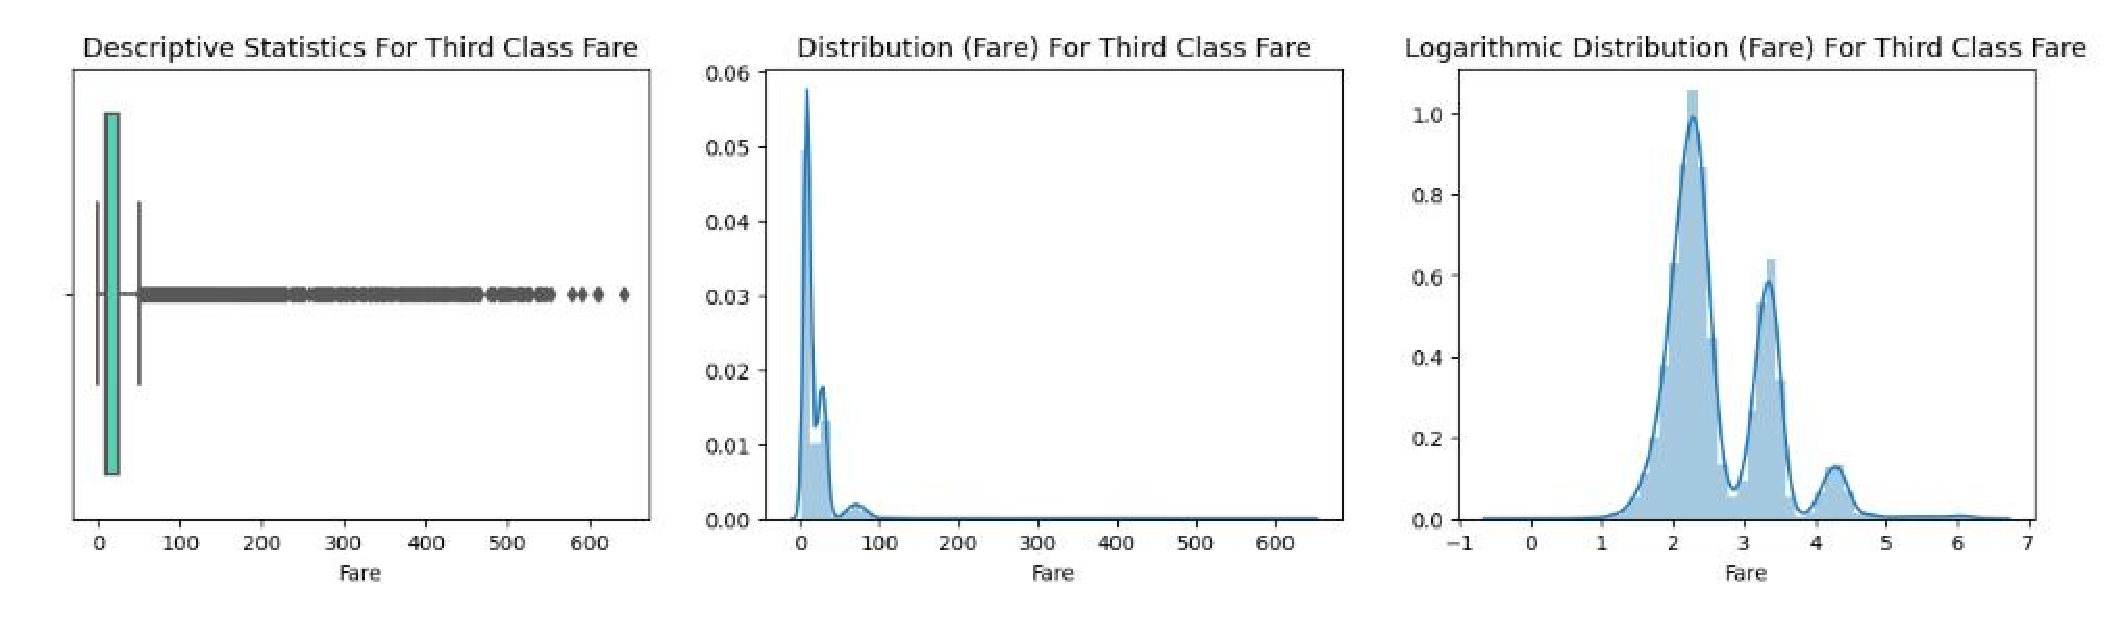
\includegraphics[width=1\textwidth]{figures//fig4.eps}\\
			\caption{Third Class Fare}
		\end{figure}
		\vspace{-0.8cm}
		\begin{center}
			\fbox{ 
				\parbox{0.86\textwidth}{ 
					\begin{center}
						As you can see from the graph, Fare does not have a fixed price for any class, so it is intended to scale the data and then use the average to impute.
					\end{center}
				} 
			}
		\end{center}
	\end{slide}
	%%
	%%==========================================================================================
	
	
	%%==========================================================================================
	%%
	\begin{slide}[toc=,bm=]{}
		Age
		\vspace{-0.8cm}
		\begin{figure}
			\centering
			\selectcolormodel{rgb}
			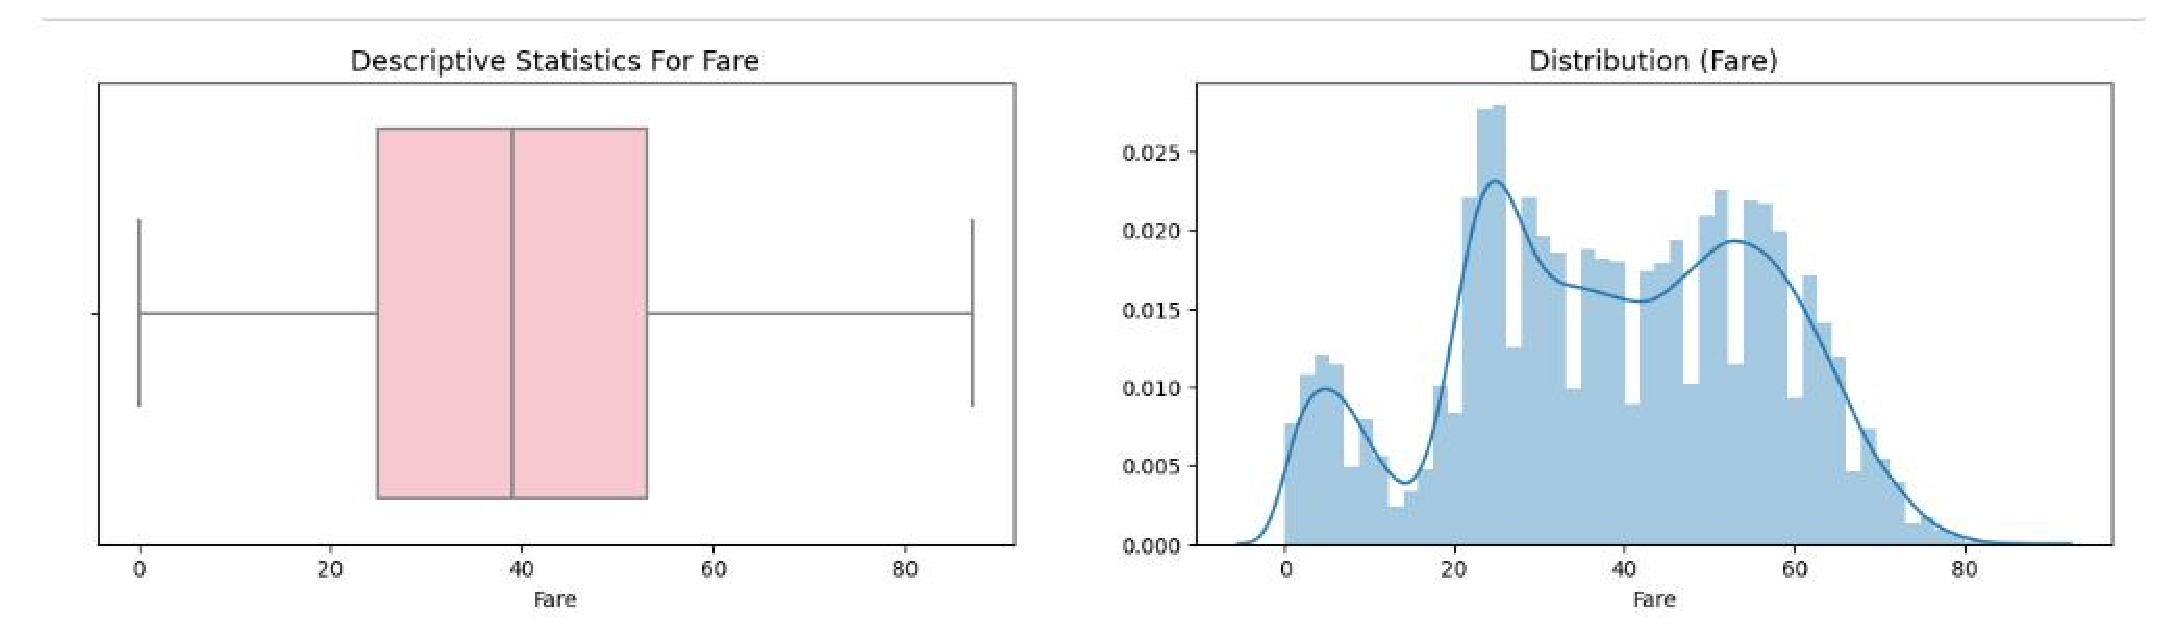
\includegraphics[width=1\textwidth]{figures//fig5.eps}\\
			\caption{Descriptive Statistics For Age}
		\end{figure}
		\begin{itemize}
			\item
			It can be seen from the figure that the missing value can be filled by the median.
		\end{itemize}
	\end{slide}
	%%
	%%==========================================================================================
	
	
	%%==========================================================================================
	%%
	\begin{slide}{Imputing Values}
		
		\begin{itemize}
			\item
			We will use \textcolor{orange}{KNN} to perform missing interpolation for Embarked.
		\end{itemize}
		\begin{center}	\begin{tabular}{c|c}
				\toprule
				%\centering
				\midrule
				{PassengerId}
				&  {$0$} \\
				{Survived}
				&  {$0$} \\
				{Pclass}
				&  {$0$} \\
				{Name}
				&  {$0$} \\
				{Sex}
				&  {$0$} \\
				{Age}
				&  {$0$} \\
				{SibSp}
				&  {$0$} \\
				{Parch}
				&  {$0$} \\
				{Ticket}
				&  {$4623$} \\
				{Fare}
				&  {$0$} \\
				{Cabin}
				&  {$67866$} \\
				{Embarked}
				&  {$0$} \\
				\bottomrule
			\end{tabular}
		\end{center}
		
	\end{slide}
	%%
	%%==========================================================================================
	
	
	%%==========================================================================================
	%%
	\begin{slide}[toc=,bm=]{Transformation and Correlations With Target Variable}
		\vspace{-0.6cm}
		\begin{figure}
			\centering
			\selectcolormodel{rgb}
			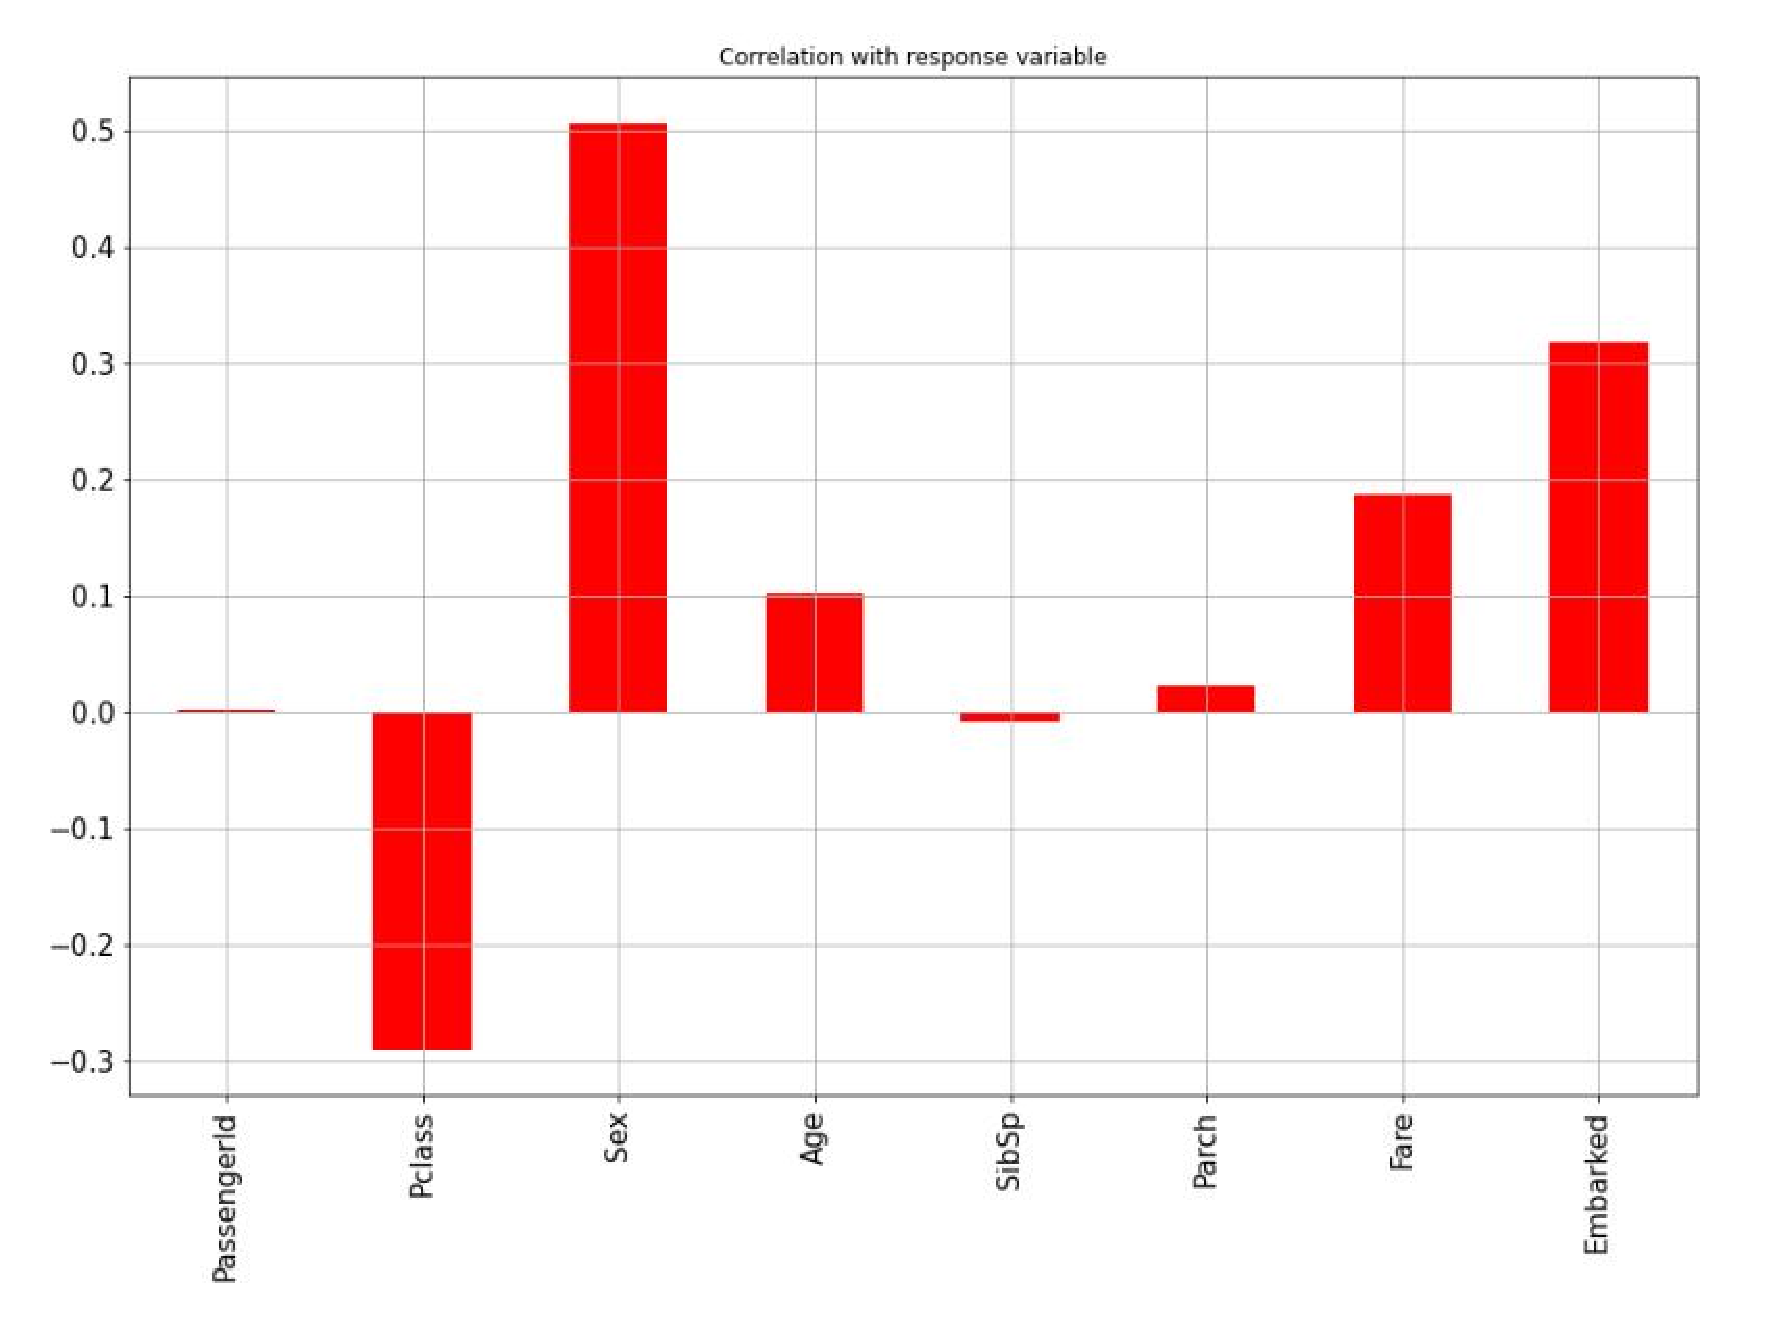
\includegraphics[width=0.6\textwidth]{figures//fig6.eps}\\
			\caption{Transformation and Correlations With Target Variable}
		\end{figure}
		\begin{itemize}
			\item
			from this we can see that variables \textcolor{orange}{SibSp, Parch , PassengerId} have a very small correlation coefficient as compared to others. We will be dropping these variables.
		\end{itemize}
		
	\end{slide}
	%%
	%%==========================================================================================
	
	
	%%==========================================================================================
	%%
	\begin{slide}[toc=,bm=]{}
		\vspace{-0.6cm}
		\begin{itemize}
			\item 
			Scale the data of Age and Fare so that all variables are in almost the same range.
		\end{itemize}
		\begin{center}
			\begin{tabular}{c| c c c c c}
				\toprule
				%\centering
				{}  & \texttt{Pclass} & \texttt{Sex}  & \texttt{Age} & \texttt{Fare}  & \texttt{Embarked}\\
				\midrule
				$0$
				&  {$1$} &  {$0$} &  {$0.034609$} &  {$-0.241265$} &  {$0.0$} \\
				$1$
				&  {$3$} &  {$0$} &  {$0.034609$} &  {$-0.439429$} &  {$0.0$} \\
				$2$
				&  {$3$} &  {$0$} &  {$-2.112537$} &  {$0.393176$} &  {$0.0$} \\
				$3$
				&  {$3$} &  {$0$} &  {$-1.075888$} &  {$-0.443884$} &  {$0.0$} \\
				$4$
				&  {$3$} &  {$0$} &  {$-0.742739$} &  {$-0.519758$} &  {$0.0$} \\
				\bottomrule
			\end{tabular}
		\end{center}	
	\end{slide}
	%%
	%%==========================================================================================
	
	
	\section{ML Models Implementation}
	
	
	%%==========================================================================================
	%%
	\begin{slide}{Overall steps}
		\begin{itemize}
			\item
			First, we set up several classifier models to make a prediction. Then we use the training set to fit the model I built. After fitting, I use the fitted model to predict the remaining data in the training set and calculate its accuracy, weight, etc. Then fuse multiple groups of models, stack the fused model with the logistic regression model, and then fit the training set to get the prediction score. Use this model to predict our test set and see the prediction results of our test set.
		\end{itemize}
	\end{slide}
	%%
	%%==========================================================================================
	
	
	%%==========================================================================================
	%%
	\begin{slide}{Step One - LogisticRegression Model.}
		\begin{itemize}
			\item
			\smallskip
			We will first split them and then fit the models.
		\end{itemize}
		\begin{figure}
			\centering
			\selectcolormodel{rgb}
			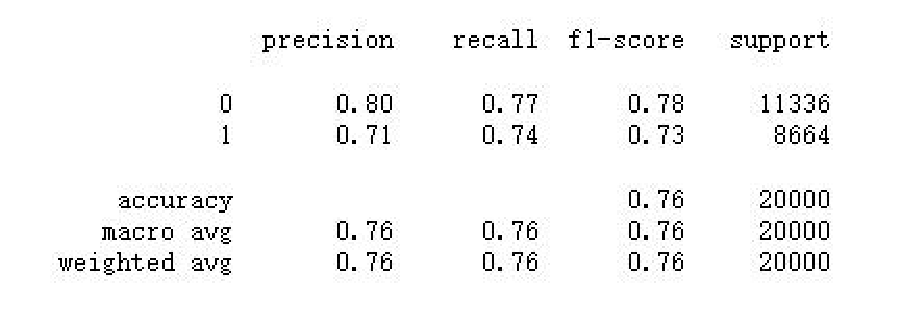
\includegraphics[width=0.8\textwidth]{figures//fig7.eps}\\
			\caption{LogisticRegression}
		\end{figure}
	\end{slide}
	%%
	%%==========================================================================================
	
	
	%%==========================================================================================
	%%
	\begin{slide}{Step Two - DecisionTreeClassifier Model}
		\begin{figure}
			\centering
			\selectcolormodel{rgb}
			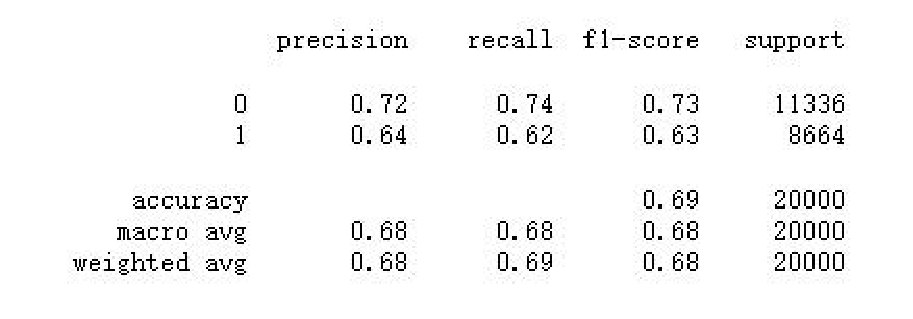
\includegraphics[width=0.8\textwidth]{figures//fig8.eps}\\
			\caption{LogisticRegression}
		\end{figure}
	\end{slide}
	%%
	%%==========================================================================================
	
	
	%%==========================================================================================
	%%
	\begin{slide}{Step There - KNeighborsClassifier Model}
		\begin{figure}
			\centering
			\selectcolormodel{rgb}
			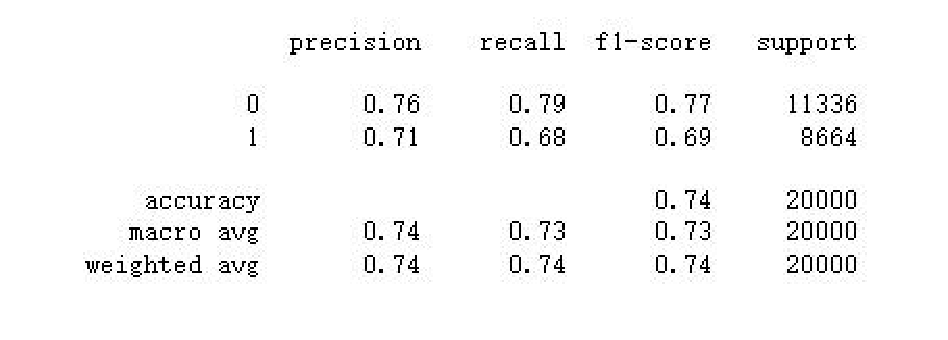
\includegraphics[width=0.8\textwidth]{figures//fig9.eps}\\
			\caption{LogisticRegression}
		\end{figure}
	\end{slide}
	%%
	%%==========================================================================================
	
	
	%%==========================================================================================
	%%
	\begin{slide}{Step Four - RandomForestClassifier Model}
		\begin{figure}
			\centering
			\selectcolormodel{rgb}
			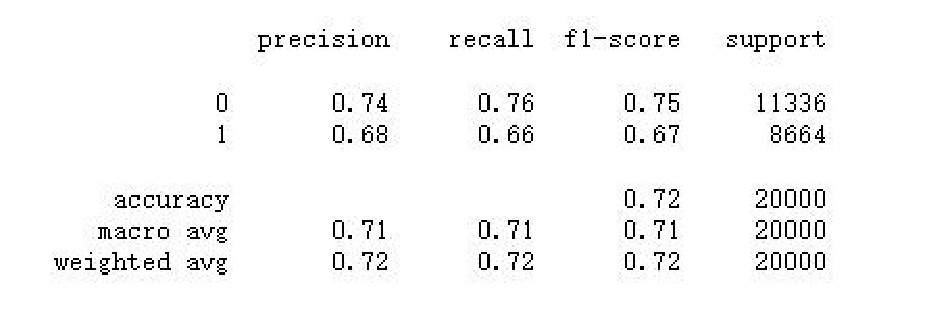
\includegraphics[width=0.8\textwidth]{figures//fig10.eps}\\
			\caption{LogisticRegression}
		\end{figure}
	\end{slide}
	%%
	%%==========================================================================================
	
	
	%%==========================================================================================
	%%
	\begin{slide}{Step Five - Stacking Classifier}
		
		\begin{itemize}
			\item
			\smallskip
			we try Stacking Classifier and Logistic Regression on the test data.
		\end{itemize}
		\begin{figure}
			\centering
			\selectcolormodel{rgb}
			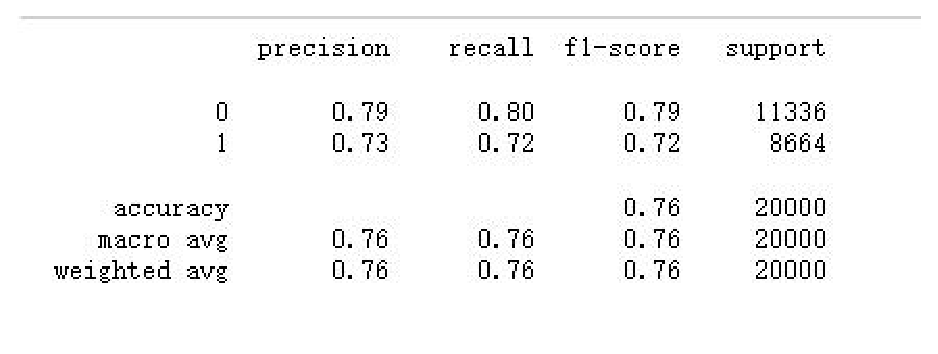
\includegraphics[width=0.8\textwidth]{figures//fig11.eps}\\
			\caption{LogisticRegression}
		\end{figure}
	\end{slide}
	%%
	%%==========================================================================================
	
	
	%%==========================================================================================
	%%
	\begin{slide}{Implementing it on Test Data}	
		\begin{itemize}
			\item
			\smallskip
			First, let's see if there are missing values in the test, and fill in the missing values in the test in the same way as train. Finally, the well-fitting model is used to make predictions.
		\end{itemize}
		\vspace{-0.6cm}
		\begin{center}	\begin{tabular}{c|c}
				\toprule
				%\centering
				\midrule
				{PassengerId}
				&  {$0$} \\
				{Survived}
				&  {$0$} \\
				{Pclass}
				&  {$0$} \\
				{Name}
				&  {$0$} \\
				{Sex}
				&  {$0$} \\
				{Age}
				&  {$3487$} \\
				{SibSp}
				&  {$0$} \\
				{Parch}
				&  {$0$} \\
				{Ticket}
				&  {$5181$} \\
				{Fare}
				&  {$133$} \\
				{Cabin}
				&  {$70831$} \\
				{Embarked}
				&  {$277$} \\
				\bottomrule
			\end{tabular}
		\end{center}
	\end{slide}
	%%
	%%==========================================================================================
	
	
	\section{Conclusion}
	
	%%==========================================================================================
	%%
	\begin{slide}{Conclusion}
		\begin{itemize}
			\item
			\smallskip
			Finally, the highest accuracy in LogisticRegression Model is 0.76.
			
			\item
			\smallskip
			A relatively basic Kaggle project was selected, the purpose is to be familiar with the Kaggle project, deeply analyze and understand each line of the project process, this project has done more processing on the step of data feature processing, and learned a lot from it
			
			\item
			\smallskip
			The work can also be further refined to improve the accuracy of prediction, for example, in the process of processing the age column, the age can be segmented according to the size of the age, and it is felt that the size of the age has a certain relationship with the size of the final survival rate.
			
		\end{itemize}
	\end{slide}
	%%
	%%==========================================================================================
	
	
	%%==========================================================================================
	% TODO: Contact Page
	\begin{wideslide}[toc=,bm=]{Contact Information}
		\centering
		\vspace{\stretch{1}}
		\twocolumn[
		lcolwidth=0.35\linewidth,
		rcolwidth=0.65\linewidth
		]
		{
			% \centerline{
\includegraphics[scale=.2]{tulip-logo.eps}}
		}
		{
			\vspace{\stretch{1}}
			jinzhu Liu\\
			Nanjing University of Science and Technology\\
			Deakin University, Australia
			\begin{description}
				\item[\textcolor{orange}{\faEnvelope}] \href{mailto:jinz_liu@njust.edu.cn}
				{\textsc{\footnotesize{jinz_liu@njust.edu.cn}}}
				
				\item[\textcolor{orange}{\faHome}] \href{http://www.tulip.org.au}
				{\textsc{\footnotesize{Team for Universal Learning and Intelligent Processing}}}
			\end{description}
		}
		\vspace{\stretch{1}}
	\end{wideslide}
	
\end{document}

\endinput
